Le domaine de compression des graphes est un domaine qui a connu une grande évolution vu son importance. Une multitude de méthodes ont été proposées au cours des dernières années, ces méthodes diffèrent l'une de l'autre dans plusieurs points comme: le type de graphe en entrée, le type de structure en sortie, le type de compression et la technique utilisée pour la compression. En se basant sur ces différences, plusieurs classifications ont été suggérées. Nous allons dans ce qui suit présenter les plus importantes parmi ces classifications.\\

Dans \citep{maneth2015survey}, les auteurs proposent une classification basée au début sur le type de compression, ils regroupent les méthodes en deux catégories principales : méthodes de compression sans perte et méthodes de compression avec perte. Les méthodes de compression sans perte sont divisées à leurs tour en trois classes selon le type de structures récupérées en sortie. La première classe est la représentation succincte, les méthodes de cette classe représentent le graphe sous forme d'une chaine de bits succincte irréversible lors de la décompression, la sortie de ces méthodes est une structure compacte du graphe originale. Parmi les méthode de cette classe, nous trouvons : Web Framework de Boldi et Vigna \citep{boldi2004webgraph}. La deuxième classe est la représentation structurelle. Contrairement à l'approche précédente, les méthodes de cette classe modifient la structure du graphe initial, sachant que les modifications apportées sont réversibles. La sortie sera donc une structure réduite et non pas compacte de la version initial. Entre ces méthodes, nous citons : RePair de Claude et Navarro \citep{claude2010fast}. La dernière catégorie est la compression RDF qui est assez récente. Les méthodes de cette classe sont appliquées sur les bases de donnés RDF, nous trouvons parmi ces techniques : Dcomp de \citep{martinez2012compression} . Les méthodes de compression avec perte quand à eux apportent des modifications irréversibles sur le graphe en supprimant les informations redondantes et le bruit. Comme exemple, nous citons : ASSG de \citep{zhang2014assg}.\\

Une autre classification a été exposée par Lui et al. dans \citep{liu2018graph} qui classe les méthodes sur trois niveaux. Au premier et deuxième niveaux, les techniques de compression sont regroupées en fonction du type de graphe en entrée selon deux critères : graphe statique ou dynamique et graphe simple ou étiqueté. Pour le troisième niveau, les auteurs catégorisent les méthodes selon la technique de traitement utilisée. Quatre catégories sont définies: les méthodes de regroupement ou agrégation, ces méthodes permettent d'agréger de manière récursive un ensemble de nœuds ou liens ou carrément un cluster en un super nœud ou un nœud virtuel, comme exemple de ces techniques, nous trouvons Grass \citep{lefevre2010grass}. Le deuxième type de méthodes sont les méthodes de compression de bits, ces méthodes minimisent le nombre de bits nécessaires au stockage du graphe en se basant sur le principe de description minimal MDL, elles peuvent être sans ou avec perte, parmi eux, nous citons LSH-based \citep{khan2014set}. La troisième classe est les méthodes de simplification qui suppriment les arrêtes inutiles et inintéressantes, entres ces méthodes, nous trouvons \citep{shen2006visual}. La dernière catégorie est l'influence, les méthodes de cette catégorie décrivent le graphe par les flux d'influence les plus importantes ce qui permet de l'analyser plus facilement, ces méthodes permettent de formuler le problème de compression comme un processus d'optimisation dans lequel la quantité de données liée à l'influence est maintenue en sortie, parmi ces technique, nous motionnons \citep{shi2015vegas}.\\


La dernière classification que nous allons voir est la classification proposée dans le master de l'année passée par Belhocine et Guermah \citep{master2017}. Cette classification s'appuie sur les taxonomies des différentes techniques de compression existantes dans la littérature en se basant sur les classifications précédentes. Elle regroupe six classes de méthodes :  basées sur l'ordre des nœuds en exploitant les principes de similarité et de localité du graphe, basées sur l'ordre des nœuds en exploitant la linéarisation du graphe, basées sur l'étiquetage des nœuds par intervalles, basées sur l'agrégation des nœuds, basées sur agrégation des liens. 

Après l'étude des méthodes basées sur l'agrégation par extraction de motifs, nous avons constaté que certaines classes ne sont pas bien définit. Les imperfections que nous avons remarqué peuvent être énumérer dans ce qui suit : 1) les méthodes d'extraction de motifs englobent certaines méthodes d'agrégation et non pas le contraire, 2) Les méthodes d'extraction de motifs ne sont pas toutes des méthodes agrégatives, nous trouvons parmi elles d'autres méthodes basées sur un vocabulaire. Nous avons donc apporté des modifications sur cette classification. La figure ci-dessous représente la classification de l'année passé après raffinement où nous avons marqué nos apports en rouge.

 \begin{figure}[H]
		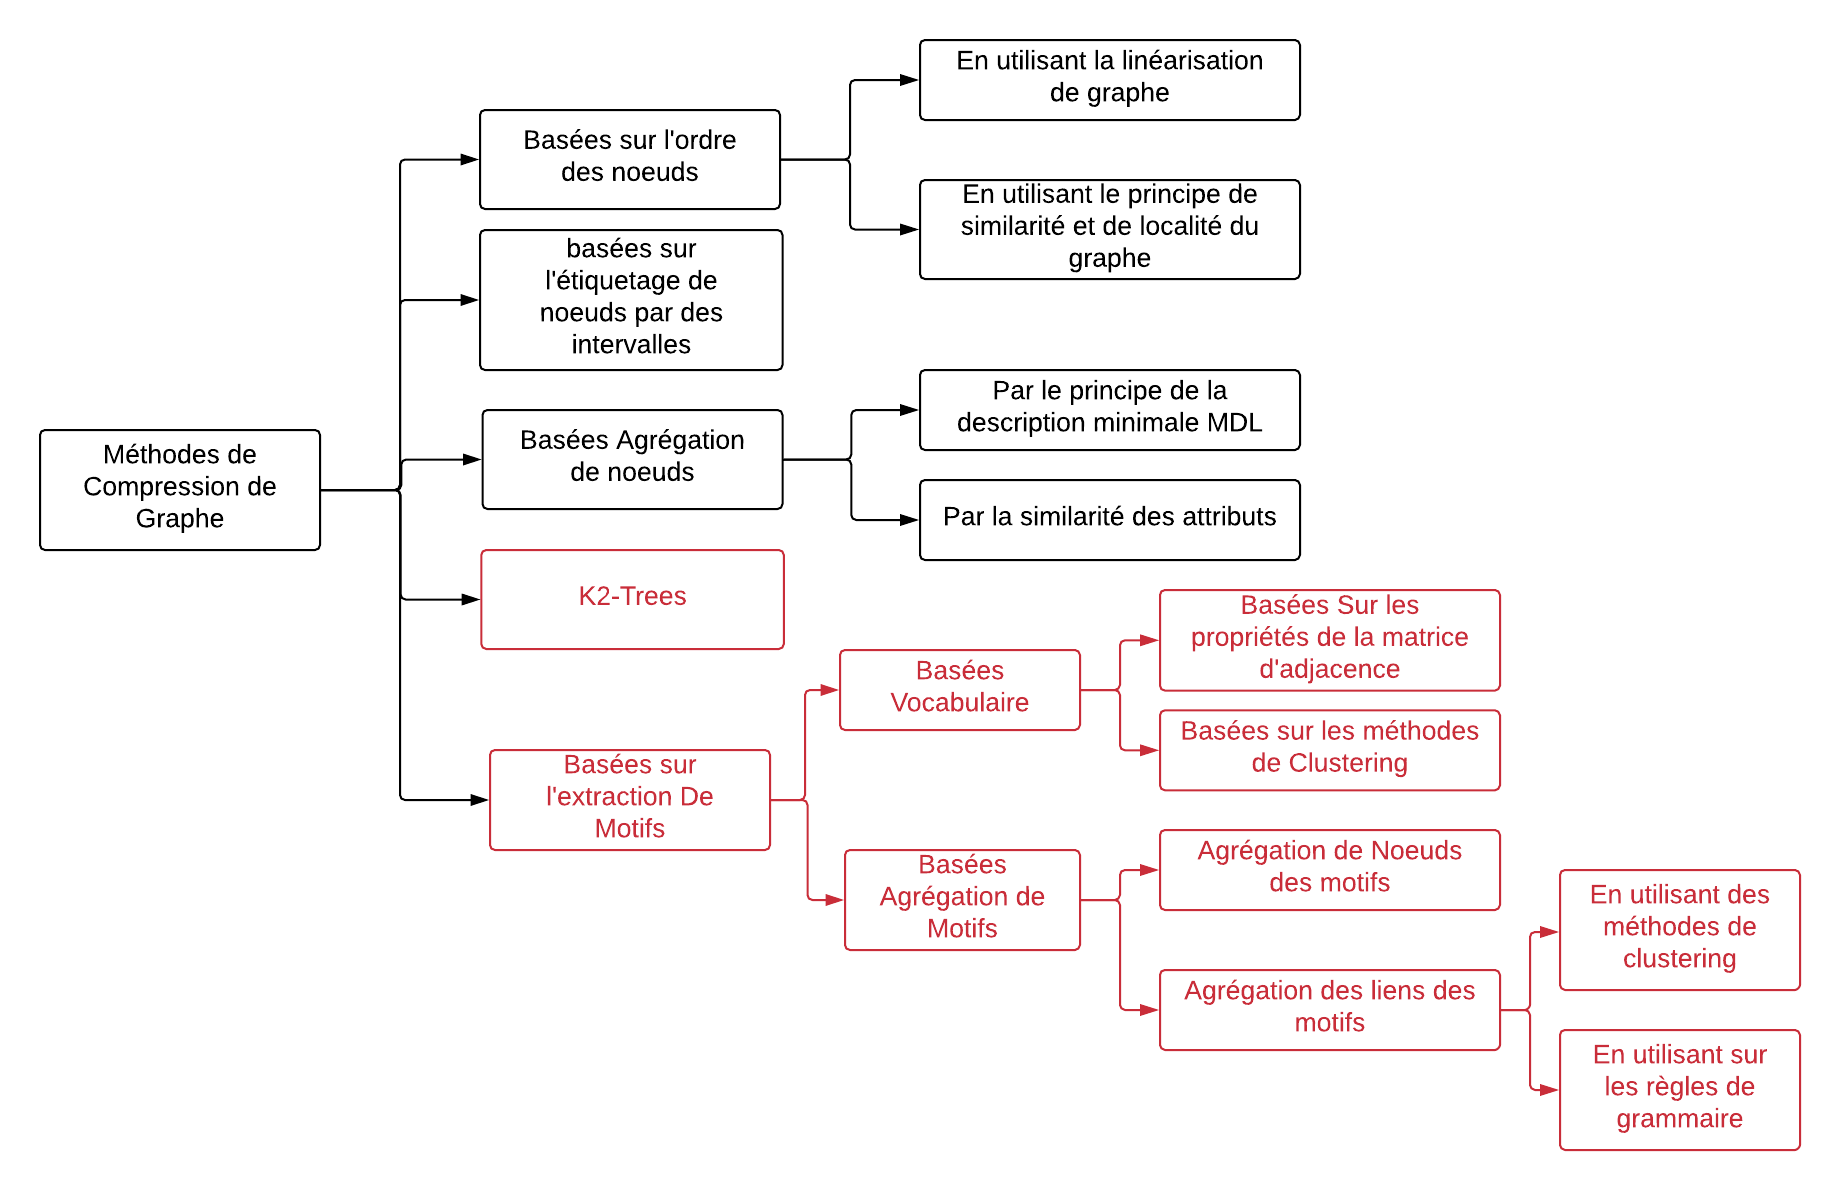
\includegraphics[scale=0.6]{./ressources/image/classif.png}
		\caption{Classification proposées des méthodes de compression}
	\end{figure}





